\chapter{Appendix - Utveckling av artificiell intelligens}

Appendix C samlar information och härledningar som ansågs viktig, men inte nödvändig, för att framföra huvudpoängen med arbetet. Först presenteras en utförlig beskrivning av rådatan arbetet omfattade. Sedan presenteras en härledning av förlustfunktion för implementering av aleatoriskosäkerhet. Därefter kommer en mer ingående beskrivning av de nätverksarkitekturer vi implementerade i arbetet. Tillsist kommer diagram från vår statistiska dataanalys som beskriver regressionslinjer beräknat från korrelationerna mellan våra valda egenskaper och tentamensresultat.

\section{Databeskrvning}
\label{app: dataDescription}

Nedan beskrivs den exakta mängden rådata som arbetet har omfattat. Till de presenteras även det ursprungliga formatet på rådatan från OpenTA samt YATA. Alla student$-$ID:n samt uppgifts$-$ID:n har genomgått en hashfunktion för att hålla individerna anonyma. De hashade ID:na mappar ett till ett med en individ eller uppgift vilket möjliggjorde att integriteten hos individen kunde bibehållas samtidigt som rådatan kunde jämföras relativt sig själv. Alla hashvärden har kortats ned till 6 karaktärer i tabellerna.


\begin{table}[hbtp]
\begin{tabular}{|l|l|l|l|l|l|}
\hline
\textbf{Platform} & \multicolumn{1}{r|}{\textbf{Kurs kod}} & \textbf{Kurs namn i arbetet} & \textbf{År}   & \textbf{Antal datarader} & \textbf{Antal studenter} \\ \hline
OpenTA   & FFM521                        & Kurs A             & 2017 & 68608           & 152             \\ \hline
OpenTA   & FFM234                        & Kurs B             & 2018 & 20422           & 101             \\ \hline
YATA     & TMS064                        & Kurs C             & 2019 & 1698             & 17              \\ \hline
\end{tabular}
\caption{Den totala mängden rådata som arbetet omfattade.}
\end{table}

\begin{table}[hbtp]
\begin{tabular}{|l|l|l|l|l|}
\hline
\textbf{user\_hash}            & \textbf{exercise\_hash}        & \textbf{question\_key} & \textbf{correct\_ans} & \textbf{timestamp}                        \\ \hline
iunjuT... & uDRbrk... & 0            & false       & 2017-04-30,13:20:03.381000+00:00 \\ \hline
\end{tabular}
\caption {Formatet på rådatan från OpenTA. En sådan rad är ekvivalent med att en student har gjort ett försök på en uppgift i OpenTA.}
\end{table}

%\begin{table}[hbtp]
%\begin{tabular}{|l|l|}
%\hline
%textbf{course\_year} & TMS064\_2019             \\ \hline
%\textbf{user\_id}     & iunjuT...                \\ \hline
%\textbf{exercise\_id} & uDRbrk...                \\ \hline
%\textbf{question\_id} & W3qoEA...                \\ \hline
%\textbf{user\_ans}    & b+3*c*t                  \\ \hline
%\textbf{facit\_ans}   & 2*b+6*c*t                \\ \hline
%\textbf{correct\_ans} & false                    \\ \hline
%\textbf{timestamp}    & 2019-04-17 13:08:25.280  \\ \hline
%\end{tabular}
%\caption{Formatet på rådatan från YATA. En sådan rad är ekvivalent med att ens student har gjort ett försök på en uppgift. (raden har transponerats av platsskäl)}
%\end{table}

\begin{table}[hbtp]
\begin{tabular}{|l|l|l|ll}
\hline
\textbf{user\_id}     & \textbf{exercise\_id} & \textbf{question\_id} & \multicolumn{1}{l|}{\textbf{correct\_ans}} & \multicolumn{1}{l|}{\textbf{timestamp}}      \\ \hline
iunjuT...  & uDRbrk...  & W3qoEA...  & \multicolumn{1}{l|}{false}                  & \multicolumn{1}{l|}{2019-04-17 13:08:25.280} \\ \hline
\textbf{course\_year} & \textbf{user\_ans}    & \textbf{facit\_ans}   &                                            &                                              \\ \cline{1-3}
TMS064\_2019          & b+3*c*t             & 2*b+6*c*t             &                                            &                                              \\ \cline{1-3}
\end{tabular}
\caption{Formatet på rådatan från YATA. En sådan rad är ekvivalent med att en student har gjort ett försök på en uppgift i YATA. I tillägg till informationen som finns i OpenTA rådatan finns här även: Kursnamn med år, vad användaren svarade vid försöket samt vad som är korrekt svar på uppgiften.}
\end{table}




\newpage

\section{Härledning av förlustfunktion för implementering av aleatorisk osäkerhet}
\label{app: derivation}
Nedan följer en härledning av två olika förlustfunktioner som implementerar aleatorisk osäkerhet. De två förlustfunktionerna uppkommer som en konsekvens av två olika antaganden av sannolikhetsfördelningar som nedan delas in i två fall.

Definiera indatamängden $\mathbb{X} = \{\mathbf{x_1},..., \mathbf{x_n}\}$ och utdatamängden $\mathbb{Y} = \{y_1,..., y_n\}$ för ett skalärt regressionsproblem. Notera att fetstilade symboler innebär tensorer av rank större än 0 och ej fetstilade tecken symboliserar tensorer av rank 0.  Låt funktionen för ett godtyckligt neuralt nätverk vara $f^\mathbf{W}$ med vikter och tröskelvärden $\mathbf{W}$. Nätverkets förutsägelse $\hat{y}_i$ givet indata $\mathbf{x_i}$ ges därmed av $\hat{y}_i = f^\mathbf{W}(\mathbf{x}_i)$.

Vårt mål är att optimera vikterna $\mathbf{W}$ vilka minimerar felet i förutsägelse $E = \sum_{i=1}^n \left\|y_i - \hat{y}_i\right\|_M$ för någon metrik $M$ samt approximera den aleatoriska osäkerheten $\sigma_x$.  Vi söker därför en förlustfunktion $\mathcal{L}(\mathbf{W})$ sådan att $\hat{y}$ och $\sigma_x$ ges som utdata av det neurala nätverket. För detta syfte applicerar vi maximum likelihood metoden. Inför därför likelihooden $p\left(y_i|f^\mathbf{W}(x_i)\right)$ samt bilda log-likelihooden $\ell(\mathbf{W}) = \log \left[p\left(y_i|f^\mathbf{W}(\mathbf{x_i})\right)\right]$. Definiera förlustfunktionen $\mathcal{L}(\mathrm{W})$ som 
\begin{equation}
    \mathcal{L}(\mathbf{W}) = -\ell(\mathbf{W}) = -\log \left[p\left(y_i|f^\mathbf{W}(\mathbf{x_i})\right)\right],
\label{eq:def_loss_fcn}
\end{equation}
ty att maximera $\ell(\mathbf{W})$ är ekvivalent med att minimera $\mathcal{L}(\mathbf{W})$.

Antag två fall för slumpvariablerna $\mathbf{X}$ och $\mathbf{Y}$ motsvarande observerad indata $\mathbf{x}$ respektive utdata $\mathbf{y}$. För att förenkla notationen utelämnas härifrån index $i$ och låt $\sigma(\mathbf{x}) = \sigma_\mathbf{x}$. Fall 1: givet $\mathbf{X}$, antag normalfördelad utdata
\begin{equation}
     \mathbf{Y} \sim \mathcal{N}\left(f^\mathbf{W}(\mathbf{X}),\, \sigma^2(\mathbf{X})  \right) \Rightarrow p\left(y|f^\mathbf{W}(\mathbf{x})\right) = \frac{1}{\sqrt{2\pi\sigma^2_x}} \exp \left\{-\frac{\left[y - f^\mathbf{W}(\mathbf{x})\right]^2}{2\sigma^2_x}\right\},\, \mathbf{x} \in \mathbb{R}.
\end{equation}
\begin{equation}
   \Rightarrow \ell(\mathbf{W}) = \log \left[p\left(y|f^\mathbf{W}(\mathbf{x})\right)\right] = \log \left[ \frac{1}{\sqrt{2\pi\sigma^2_x}}\right] - \frac{\left[y - f^\mathbf{W}(\mathbf{x})\right]^2}{2\sigma^2_x}
\end{equation}
\begin{equation}
    \Rightarrow \ell(\mathbf{W}) = -\frac{1}{2} \left[\log 2\pi + \log \sigma_x^2 + \exp{\left(-\log \sigma_x^2 \right)} \left|y - f^\mathbf{W}(\mathbf{x})\right|^2 \right]
\label{eq:const_arg}
\end{equation}
Eftersom konstanta termer som $\log 2\pi$ och konstanta faktorer som $\frac{1}{2}$ ej påverkar optimeringsproblemet kan vi sätta
\begin{equation}
    \ell(\mathbf{W}) = -\left[\log \sigma_x^2 + \exp{\left(-\log \sigma_x^2 \right)} \left|y - f^\mathbf{W}(\mathbf{x})\right|^2 \right].
\end{equation}
Därmed erhålls enligt ekvation \eqref{eq:def_loss_fcn}
\begin{equation}
    \mathcal{L}_{\mathrm{normal}}(\mathbf{W}) = \exp{\left(-\log \sigma_x^2 \right)} \left\|y - f^\mathbf{W}(\mathbf{x})\right\|_2 + \log \sigma_x^2.
    \label{eq:normal_loss_fcn}
\end{equation}
Observera att införandet av $\sigma_x$ medför två effekter på förlustfunktionen. Den första är en osäkerhetsattenuationsfaktor $\exp{\left(-\log \sigma_x^2 \right)}$ som minskar bidraget av felet $\left\|y - f^\mathbf{W}(\mathbf{x})\right\|_2$ vid växande osäkerheter $\sigma_x$. För det andra införs en osäkerhetsterm $\log \sigma_x^2$ som bidrar växande till förlustfunktionen för växande $\sigma_x^2$. Notera även att vid konstant $\sigma_x^2$ återfås den kanoniska kvadratiska förlustfunktionen (eng. \emph{Mean Squared Error}, MSE) $\mathcal{L}_\mathrm{MSE}(\mathbf{W}) = \left\|y - f^\mathbf{W}(\mathbf{x})\right\|_2$.

Fall 2: givet $\mathbf{X}$, antag Laplacefördelad utdata
\begin{equation}
    \mathbf{Y} \sim \mathrm{Laplace}\left(f^\mathbf{W}(\mathbf{X}),\, \sigma(\mathbf{X}) \right) \Rightarrow p\left(y|f^\mathbf{W}(\mathbf{x})\right) = \frac{1}{2\sigma_x} \exp \left[-\frac{\left|y - f^\mathbf{W}(\mathbf{x})\right|}{\sigma_x} \right],\, \mathbf{x} \in \mathbb{R}.
\end{equation}
\begin{equation}
    \Rightarrow \ell(\mathbf{W}) = \log \left[p\left(y|f^\mathbf{W}(\mathbf{x})\right)\right] = -\left[\log 2 + \log \sigma_x + \exp{\left(-\log \sigma_x\right)}\left|y - f^\mathbf{W}(\mathbf{x})\right|\right].
\end{equation}
Analogt med ekvation \eqref{eq:const_arg} kan vi ty en konstant term $\log 2$ sätta
\begin{equation}
    \ell(\mathbf{W}) = -\left[\exp{\left(-\log \sigma_x\right)}\left|y - f^\mathbf{W}(\mathbf{x})\right| + \log \sigma_x\right].
\end{equation}
Slutligen erhålls enligt ekvation \eqref{eq:def_loss_fcn}
\begin{equation}
    \mathcal{L}_\mathrm{Laplace}(\mathbf{W}) = \exp{\left(-\log \sigma_x\right)}\left\|y - f^\mathbf{W}(\mathbf{x})\right\|_1 + \log \sigma_x.
\end{equation}
Liknande observationerna för fall 1 kan vi notera en osäkerhetsattenuationsfaktor $ \exp{\left(-\log \sigma_x\right)}$ och ett osäkerhetsbidrag $\log \sigma_x$. Observera däremot skillnaden i metrik för felet i förutsägelse $\left\|y - f^\mathbf{W}(\mathbf{x})\right\|_1$ och att för konstant $\sigma_x$ återfås det standardmässiga absolutfelet (eng. \emph{Mean Absolute Error}, MAE) $\mathcal{L}_\mathrm{MAE}(\mathbf{W}) = \left\|y - f^\mathbf{W}(\mathbf{x})\right\|_1$.

\newpage

\section{Nätverskarkitekturer}
\label{app:architecture_appendix}
Nedan presenteras en mer noggrann beskrivning av de som presenterades i sektion \ref{sec:training_and_validation}. Nätverksarkitekturerna presenteras i ordningen för respektive problem: U/G, U/3/4/5 och skrivningspoäng samt för implementering av aleatorisk osäkerhet. Den generella strukturen för nätverksarkitekturerna visas i figur \ref{fig:general_nn_app}.


\begin{figure}[hbtp]
    \centering
    \resizebox {\textwidth} {!} {
        \definecolor{input_node}{RGB}{171,171,154}
\definecolor{dense_node}{RGB}{196,225,144}
\definecolor{dropout_node}{RGB}{222,222,222}
\definecolor{output_node}{RGB}{171,154,154}
% New colors
\definecolor{klight_green_400}{RGB}{156, 204, 101}



\begin{tikzpicture}[x=1.5cm, y=1.5cm, >=stealth]
\tikzset{%
  dense neuron/.style={
    circle,
    draw,
    fill=klight_green_400,
    thick,
    minimum size=1cm
  },
  dropout neuron/.style={
    circle,
    draw,
    fill=dropout_node,
    thick,
    minimum size=1cm
  },
  input neuron/.style={
    circle,
    draw,
    fill=input_node,
    thick,
    minimum size=1cm
  },
  output neuron/.style={
    circle,
    draw,
    fill=output_node,
    thick,
    minimum size=1cm
  },
  neuron missing/.style={
    draw=none, 
    scale=4,
    fill=none,
    text height=0.333cm,
    execute at begin node=\color{black}$\vdots$
  },
}


% Input layer
\foreach \m/\l [count=\y] in {1,2,3,missing,4}
  \node [input neuron/.try, neuron \m/.try] (input-\m) at (0,2.5-\y) {};
% First dropout layer
\foreach \m/\l [count=\y] in {1,2,3,missing,4}
  \node [dropout neuron/.try, neuron \m/.try] (dropout1-\m) at (2,2.5-\y) {};
% First hidden layer
\foreach \m [count=\y] in {1,2,3,missing,4}
  \node [dense neuron/.try, neuron \m/.try ] (hidden1-\m) at (4,2.5-\y) {};
% Second dropout layer
\foreach \m/\l [count=\y] in {1,2,3,missing,4}
  \node [dropout neuron/.try, neuron \m/.try] (dropout2-\m) at (6,2.5-\y) {};
% Second hidden layer
\foreach \m [count=\y] in {1,2,3,missing,4}
  \node [dense neuron/.try, neuron \m/.try ] (hidden2-\m) at (8,2.5-\y) {};
% Output layer
\foreach \m [count=\y] in {1,missing,2}
  \node [input neuron/.try, neuron \m/.try ] (output-\m) at (10,2-1.25*\y) {};

Draw node labels
\foreach \l [count=\i] in {1,2,3,n}
  \draw [<-] (input-\i) -- ++(-1,0)
    node [above, midway] {$x_\l$};

\foreach \l [count=\i] in {1,n}
  \draw [->] (output-\i) -- ++(1,0)
    node [above, midway] {$\hat{y}_\l$};

% Draw connections
\foreach \i in {1,...,4}
    \draw [->] (input-\i) -- (dropout1-\i);
    
\foreach \i in {1,...,4}
  \foreach \j in {1,...,4}
    \draw [->] (dropout1-\i) -- (hidden1-\j);

\foreach \i in {1,...,4}
    \draw [->] (hidden1-\i) -- (dropout2-\i);
    
\foreach \i in {1,...,4}
  \foreach \j in {1,...,4}
    \draw [->] (dropout2-\i) -- (hidden2-\j);

\foreach \i in {1,2,3,...,4}
  \foreach \j in {1,2}
    \draw [->] (hidden2-\i) -- (output-\j);

\foreach \l [count=\x from 0] in {Tillplattnings-, Utsläcknings-, Dolt tätt, Utsläcknings-, Dolt tätt, Utdata-}
  \node [align=center, above] at (\x*2,2) {\textbf{\l} \\ \textbf{lager}};
  
\foreach \l [count=\x from 0] in {Varierbar storlek, , , , , 1-4 noder}
  \node [align=center, below] at (\x*2,-3) {\l};

\end{tikzpicture}
    }
    \caption{Generell nätverksarkitektur. Nätverket består av ett tillplattningslager följt av två utsläckninglager om lott med två dolda täta lager.}
    \label{fig:general_nn_app}
\end{figure}

För U/G-problemet användes en nätverksarkitektur enligt figur \ref{fig:general_nn_app}. Nätverket för U/G-problemet benämns vidare som U/G-nätverket. Indatan på matrisform omvandlades först till vektorer med hjälp av tillplattningslagret, varefter den behandlades av två dolda täta lager med 32 noder vardera med aktiveringsfunktion \emph{ReLU}. Dessa dolda täta lager var även viktregulariserade, vilket i kombination med utsläcknings-lagren innan dem motverkade överanpassning. Sista lagret var ett dolt tätt lager med en nod samt \emph{sigmoid}-aktivering, vilket gav att utvärdet från det neurala nätverket blev ett tal mellan 0 och 1. Detta tal motsvarar nätverkets uppskattade sannolikhet att en given student får godkänt i kursen. \emph{Binär entropi }(eng. \emph{Binary crossentropy}) valdes som förlustfunktion och \emph{RMSProp} valdes som optimeringsalgoritm. 

Nätverksarkitekturen för U5-problemet ges i figur \ref{fig:general_nn_app}. Nätverket benämns som U/5-nätverket och består av ett tillplatningslager samt två dolda täta lager med 16 noder vardera och \emph{ReLU}-aktivering. För att motverka överanpassning var dessa lager även viktregulariserade. Det sista lagret bestod av ett dolt tätt lager med fyra noder med \emph{softmax}-aktivering. Vardera av dessa noder kan därmed anta ett värde mellan 0 och 1 (med total summa 1 över alla fyra), vilket svarar mot nätverkets uppskattning för att en given student får ett av de fyra betygen U-5. \emph{Kategorisk entropi} (eng. \emph{Categorical crossentropy}) valdes som förlustfunktion och \emph{RMSprop} valdes som optimeringsalgoritm. 

Den generella arkitekturen i figur \ref{fig:general_nn_app} användes även för skrivningspoängsproblemet och implementeringen av aleatorisk osäkerhet. Nätverken för skrivningspoängsproblemet benämns vidare som poängnätverk och nätverken för implementeringen av aleatorisk osäkerhet namnges till osäkerhetsnätverk. Poängnätverken har en utdatanod. För kurs B bestod poängnätverket av tre dolda täta lager med 16, åtta respektive åtta noder med aktiveringsfunktion \emph{ReLU}. För att motverka överanpassning användes utsläckning för indatan till varje dolt tätt lager med utsläckningssannolikheter 0.4, 0.2 respektive 0.2. Förlustfunktionen valdes till \emph{MSE} och optimeringsalgoritmen var \emph{RMSprop}.

För kurs A bestod poängnätverket av två dolda täta lager med 32 respektive 16 noder med aktiveringsfunktion \emph{ReLU}. Utsläckning applicerades på indatan av varje tätt lager för att motverka överanpassning. Utsläckningssannolikheterna var 0.4 respektive 0.2. Analogt med nätverksarkitekturen för kurs B valdes förlustfunktionen \emph{MSE} och optimeringsalgoritmen \emph{RMSprop}.

Osäkerhetsnätverken implementerade den normalfördelade förlustfunktionen med inkluderad aleatorisk osäkerhet enligt ekvation \eqref{eq:loss_fcn}. Till skillnad mot skrivningspoängsnätverken medför inkluderandet av aleatorisk osäkerhet att osäkerhetsnätverken har två utdatanoder istället för en. Osäkerhetsnätverket för kurs A bestod av tre dolda täta lager med nodantal 16, 16 och 32 noder. Nätverket för kurs B bestod av tre dolda lager med 32, 32, respektive 64 noder. Utsläckning användes för båda osäkerhetsnätverken på indatan till varje dolt tätt lager för att minska överanpassning. För kurs A var utsläckningssannolikheterna 0.5, 0.2 och 0.1 samt för kurs B var sannolikheterna 0.45, 0.1 respektive 0.1.

\section{Diagram från statistisk dataanalys}
\label{app:diag}
Nedan följer diagram som togs fram i samband med beräkningar av korrelationer, beskriven i \ref{sec:korre}. För både kurs A och B noterar vi att avståndet mellan regressionslinjerna och punkterna är mindre för U/5 än för U/G, detta för samtliga egenskaper. Ett större avstånd för U/G än för U/5 indikerar att en regressionlinje är mer svåranpassad för en binär mängd (U/G) än för en mängd innehållandes mer än två distinkta värden. Vi observerar även att tidsegenskaper korrelerar strikt negativt med måldata medan försöksegenskaper korrelerar positivt. Till sist noterar vi att få punkter ligger längs regressionslinjerna vilket kan tyda på att en annan form av regression är mer lämplig för dessa datamängder än linjär regression.

\begin{figure}[hbtp]
    \centering
    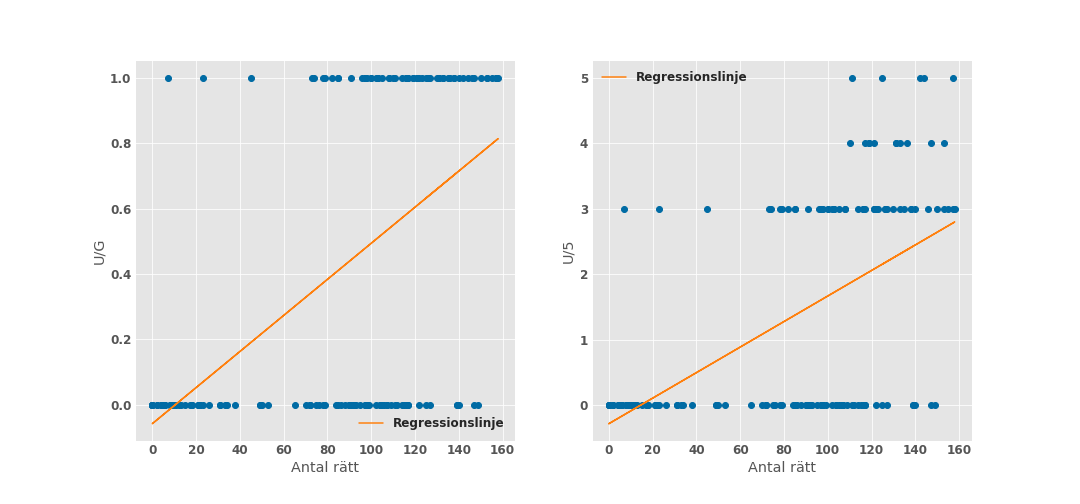
\includegraphics[width=1\textwidth]{images/pktdiagram/mekEg0.png}
    \caption{Punktdiagram för kurs A. Totalt antal rätt korrelerat mot U/G (vänster) och U/5 (höger).}
    \label{fig:pktdigA1}
\end{figure}

\begin{figure}[hbtp]
    \centering
    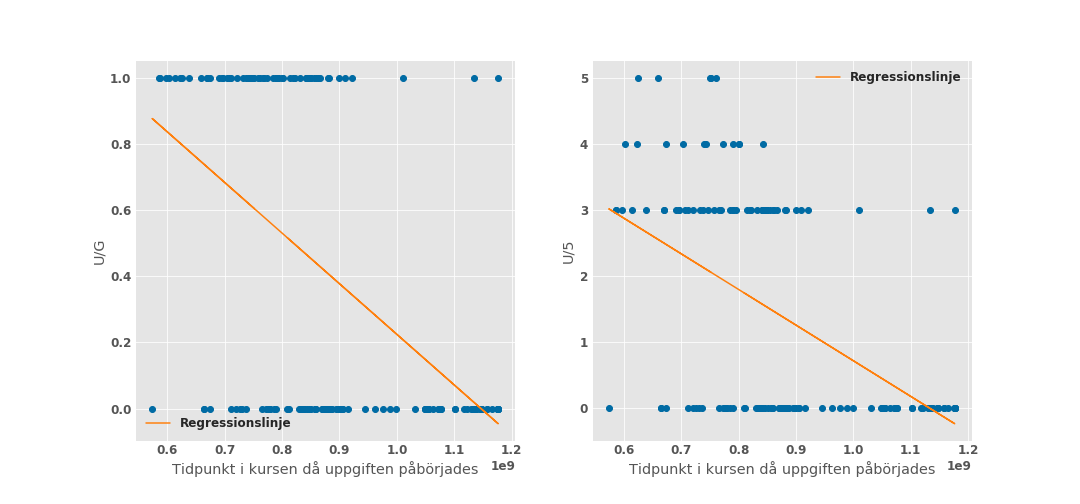
\includegraphics[width=1\textwidth]{images/pktdiagram/mekEg2.png}
    \caption{Punktdiagram för kurs A. Tidpunkt då uppgiften påbörjades korrelerat mot U/G (vänster) och U/5 (höger).}
    \label{fig:pktdigA2}
\end{figure}

\begin{figure}[hbtp]
    \centering
    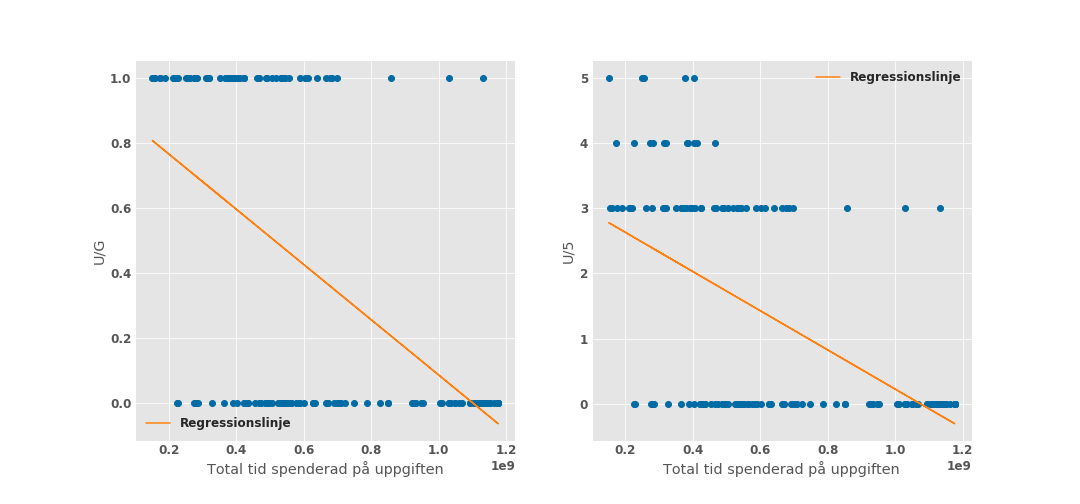
\includegraphics[width=1\textwidth]{images/pktdiagram/mekEg4.png}
    \caption{Punktdiagram för kurs A. Total spenderad tid korrelerat mot U/G (vänster) och U/5 (höger).}
    \label{fig:pktdigA3}
\end{figure}

\begin{figure}[hbtp]
    \centering
    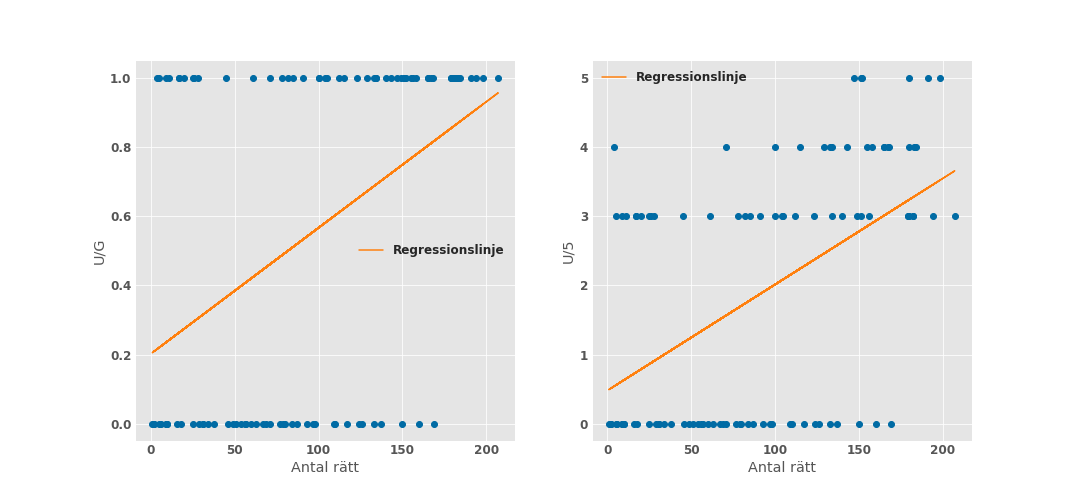
\includegraphics[width=1\textwidth]{images/pktdiagram/vektEg0.png}
    \caption{Punktdiagram för kurs B. Totalt antal rätt korrelerat mot U/G (vänster) och U/5 (höger).}
    \label{fig:pktdigB1}
\end{figure}

\begin{figure}[hbtp]
    \centering
    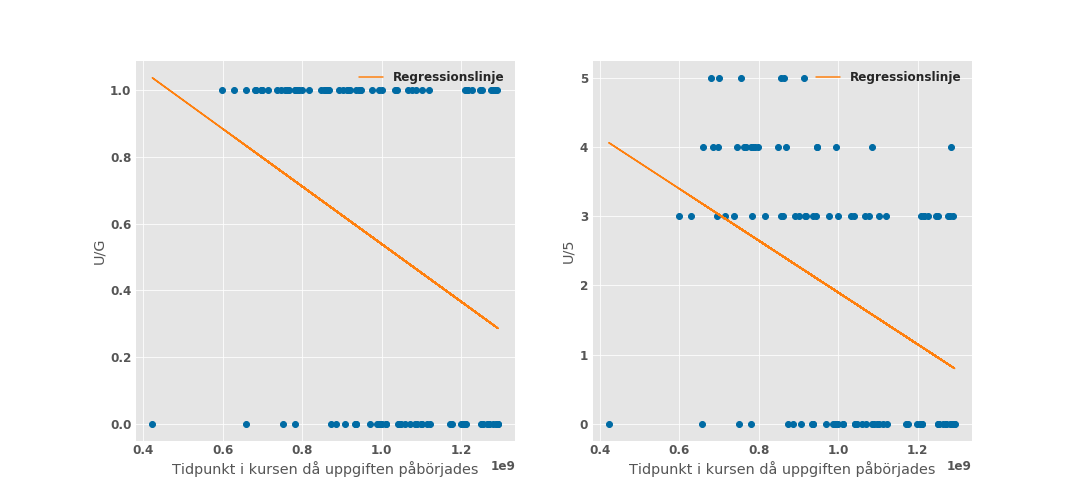
\includegraphics[width=1\textwidth]{images/pktdiagram/vektEg2.png}
    \caption{Punktdiagram för kurs B. Tidpunkt då uppgiften påbörjades korrelerat mot U/G (vänster) och U/5 (höger).}
    \label{fig:pktdigB2}
\end{figure}

\begin{figure}[hbtp]
    \centering
    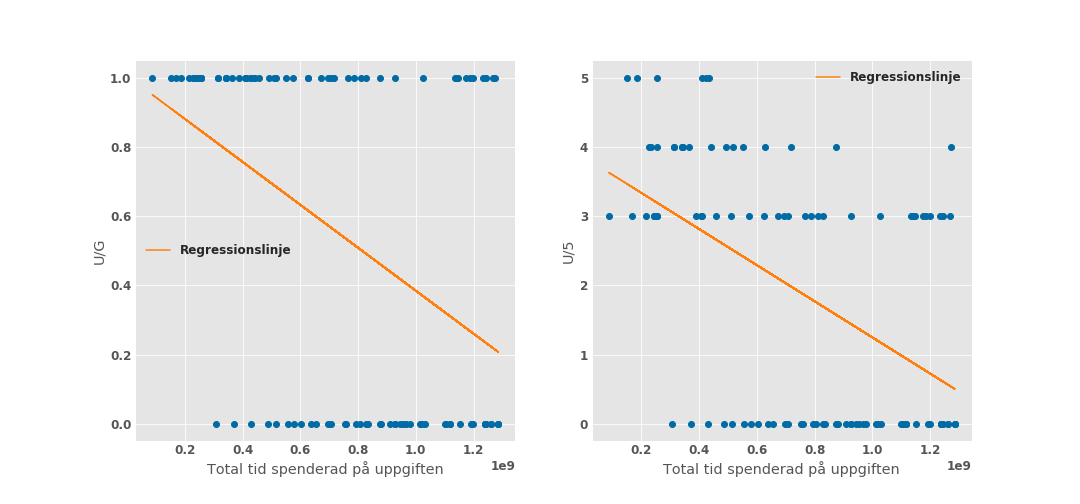
\includegraphics[width=1\textwidth]{images/pktdiagram/vektEg4.png}
    \caption{Punktdiagram för kurs B. Total spenderad tid korrelerat mot U/G (vänster) och U/5 (höger).}
    \label{fig:pktdigB3}
\end{figure}

